\documentclass[tikz]{standalone}
\usetikzlibrary {arrows.meta, angles, quotes}
\begin{document}
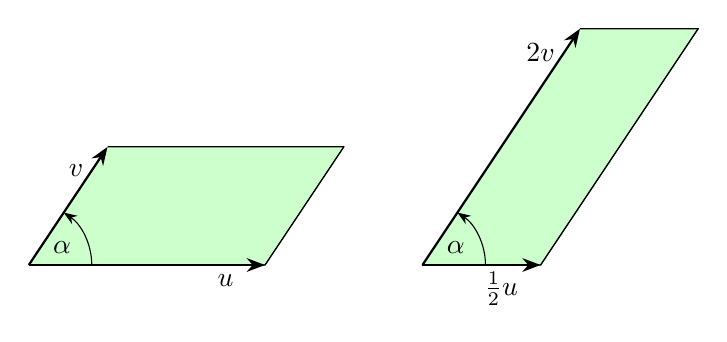
\begin{tikzpicture}[>=Stealth]
    \coordinate (A) at (0,0);
    \coordinate (B) at (3,0);
    \coordinate (C) at (4,1.5);
    \coordinate (D) at (1,1.5);

    \filldraw[fill=green!20] (A) -- (B) -- (C) -- (D);
    \draw[->, thick] (A) -- (B);
    \draw[->, thick] (A) -- (D);
    \draw (D) -- (C);
    \draw (B) -- (C);
    \node[shift={(-0.4,-0.3)}] (v) at (D) {$v$};
    \node[shift={(-0.5,-0.2)}] (u) at (B) {$u$};
    \pic ["$\alpha$", ->, draw=black, angle radius=0.8cm, angle eccentricity=0.6] {angle=B--A--D};

    \coordinate (A') at (5,0);
    \coordinate (B') at (6.5,0);
    \coordinate (C') at (8.5,3);
    \coordinate (D') at (7,3);

    \filldraw[fill=green!20] (A') -- (B') -- (C') -- (D');
    \draw[->, thick] (A') -- (B');
    \draw[->, thick] (A') -- (D');
    \draw (D') -- (C');
    \draw (B') -- (C');
    \node[shift={(-0.5,-0.3)}] (v) at (D') {$2v$};
    \node[shift={(-0.5,-0.3)}] (u) at (B') {$\frac{1}{2}u$};
    \pic ["$\alpha$", ->, draw=black, angle radius=0.8cm, angle eccentricity=0.6]
    {angle=B'--A'--D'};
\end{tikzpicture}
\end{document}
